\documentclass[varwidth,border=5pt]{standalone}

\usepackage{tikz}
\usepackage{tikz-3dplot}
\usepgflibrary{shapes.geometric}
\usetikzlibrary{calc}


\begin{document}

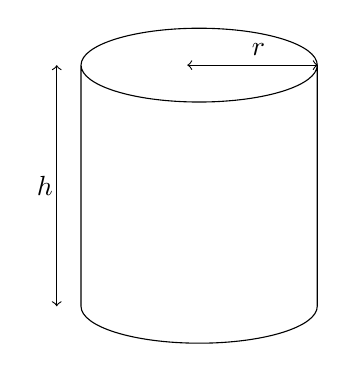
\begin{tikzpicture}
\node [draw, cylinder, shape aspect=4, rotate=90, minimum height=4cm,minimum width=3cm] (c) {};
\coordinate(htop) at ($(c.before top)!-1*.1!(c.after top)$);
\coordinate(hbot) at ($(c.after bottom)!-1*.1!(c.before bottom)$);
\coordinate(hlab) at ($(htop)!.5!(hbot)+(c.north)!.9!(c.center)$);
\draw[<->] (hbot)--(htop);
\path (hlab) node {$h$}; %Modify height label here
\coordinate (center) at ($(c.before top)!0.5!(c.after top)$);
\coordinate (rlab) at ($(center) !0.5!(c.after top)$);
\coordinate (rtop) at ($(center)!-1*.1!(c.after top)$);
\draw[<->] (rtop) -- (c.after top);
\path (rlab) node[above] {$r$}; %Modify radius label here
\end{tikzpicture}

\end{document}
